\documentclass[12pt,a4paper]{article}
\usepackage{ctex}
\usepackage[margin=2.5cm]{geometry}
\usepackage{graphicx}
\usepackage{booktabs}
\usepackage{amsmath}
\usepackage{amssymb}
\usepackage{hyperref}
\usepackage{float}
\usepackage{enumitem}
\usepackage{fancyhdr}
\usepackage{xcolor}
\usepackage{subcaption}

\graphicspath{{figures/}}

\pagestyle{fancy}
\fancyhf{}
\rhead{RA-YOLO 设计原理}
\lhead{技术决策说明}
\rfoot{\thepage}

\title{\textbf{RA-YOLO 技术决策说明书\\——为什么这么实现}}
\author{设计原理与技术选型分析}
\date{\today}

\begin{document}

\maketitle
\tableofcontents
\newpage

% ============================
\section{引言}
% ============================

这份文档从我的第一视角出发,详细说明在构建RA-YOLO遥感飞机旋转目标检测系统时,每个关键技术决策背后的思考过程和选择依据。不是简单地罗列``用了什么'',而是解释``为什么这么做''。

% ============================
\section{为什么选择旋转框(OBB)而不是水平框}
% ============================

\subsection{问题本质}

拿到这个遥感飞机检测任务后,我首先思考的是标注形式的选择。水平框(HBB)是最简单的方案,但在遥感场景下存在根本性缺陷。

飞机是一种细长型目标,长宽比通常在3:1到5:1之间。当飞机以斜45度停放时,水平框需要包含大量背景区域才能框住目标,导致:
\begin{itemize}[leftmargin=2em]
    \item 目标区域占比低(有效像素可能不到框面积的30\%)
    \item 相邻飞机的水平框严重重叠,NMS容易误抑制
    \item 无法获取飞机的朝向信息
\end{itemize}

旋转框(OBB)直接用四个顶点坐标或中心点+宽高+角度来描述目标,能紧密贴合飞机的实际轮廓。虽然增加了回归的复杂度(从4个参数变为5个或8个),但带来的定位精度提升是值得的。图\ref{fig:red_obb_why}展示了旋转框的检测效果,可以看到红色旋转框能够精确描述飞机的方向和轮廓。

\begin{figure}[H]
\centering
\includegraphics[width=0.55\textwidth]{sample_0000_red_obb.jpg}
\caption{红色旋转框检测效果。与水平框相比,旋转框紧密贴合飞机目标,减少了背景区域的干扰}
\label{fig:red_obb_why}
\end{figure}

\subsection{为什么选择四点坐标格式}

YOLO OBB支持两种标注格式:(x,y,w,h,$\theta$)和四点坐标(x1,y1,x2,y2,x3,y3,x4,y4)。我选择四点坐标格式,原因在于:
\begin{itemize}[leftmargin=2em]
    \item 避免角度表示的歧义($\theta$在0°和180°时等价,需要额外处理周期性)
    \item 四点坐标能表示任意四边形,不限于矩形,适应标注误差
    \item 与OpenCV的旋转矩形操作直接兼容
\end{itemize}

% ============================
\section{为什么选择YOLOv8-OBB作为基线框架}
% ============================

\subsection{框架对比考量}

在选择基线框架时,我对比了几个主流方案:

\begin{table}[H]
\centering
\caption{旋转目标检测框架对比}
\begin{tabular}{lccc}
\toprule
\textbf{框架} & \textbf{速度} & \textbf{精度} & \textbf{易用性} \\
\midrule
Faster R-CNN OBB & 慢 & 高 & 一般 \\
FCOS-R & 中等 & 中等 & 一般 \\
Oriented R-CNN & 慢 & 高 & 较难 \\
YOLOv8-OBB & 快 & 中高 & 好 \\
\bottomrule
\end{tabular}
\end{table}

选择YOLOv8-OBB基于以下考量:

\begin{enumerate}[leftmargin=2em]
    \item \textbf{框架成熟度}:Ultralytics的YOLOv8生态完善,训练、验证、推理、导出一站式支持
    \item \textbf{OBB原生支持}:不需要额外魔改代码,直接支持旋转框检测
    \item \textbf{速度优势}:单阶段检测器在部署场景下的速度优势明显
    \item \textbf{改进空间}:作为基线模型,有明确的改进方向(注意力、损失函数等)
    \item \textbf{双阶段对比需求}:用户需要``双阶段YOLO系列'',即基线和改进两个阶段的对比
\end{enumerate}

\subsection{关于``双阶段''的理解}

用户提到``双阶段的YOLO系列'',这里的``双阶段''并非指传统的two-stage detector(如Faster R-CNN),而是指研究范式上的两个阶段:
\begin{enumerate}[leftmargin=2em]
    \item \textbf{阶段一}:建立基线(YOLOv8-OBB标准配置),获取benchmark
    \item \textbf{阶段二}:引入改进(ASC + KPRLoss + 增强策略),验证提升效果
\end{enumerate}

这种对比式的研究方法能清晰展示每个改进模块的贡献。

% ============================
\section{为什么设计ASC注意力模块}
% ============================

\subsection{问题诊断}

分析基线模型的检测结果(如图\ref{fig:detection_why}所示),发现主要的失败案例集中在:
\begin{itemize}[leftmargin=2em]
    \item 小尺度飞机漏检(特征太弱)
    \item 密集停放区域的误检(背景干扰)
    \item 低对比度区域的定位偏差(轮廓不清晰)
\end{itemize}

\begin{figure}[H]
\centering
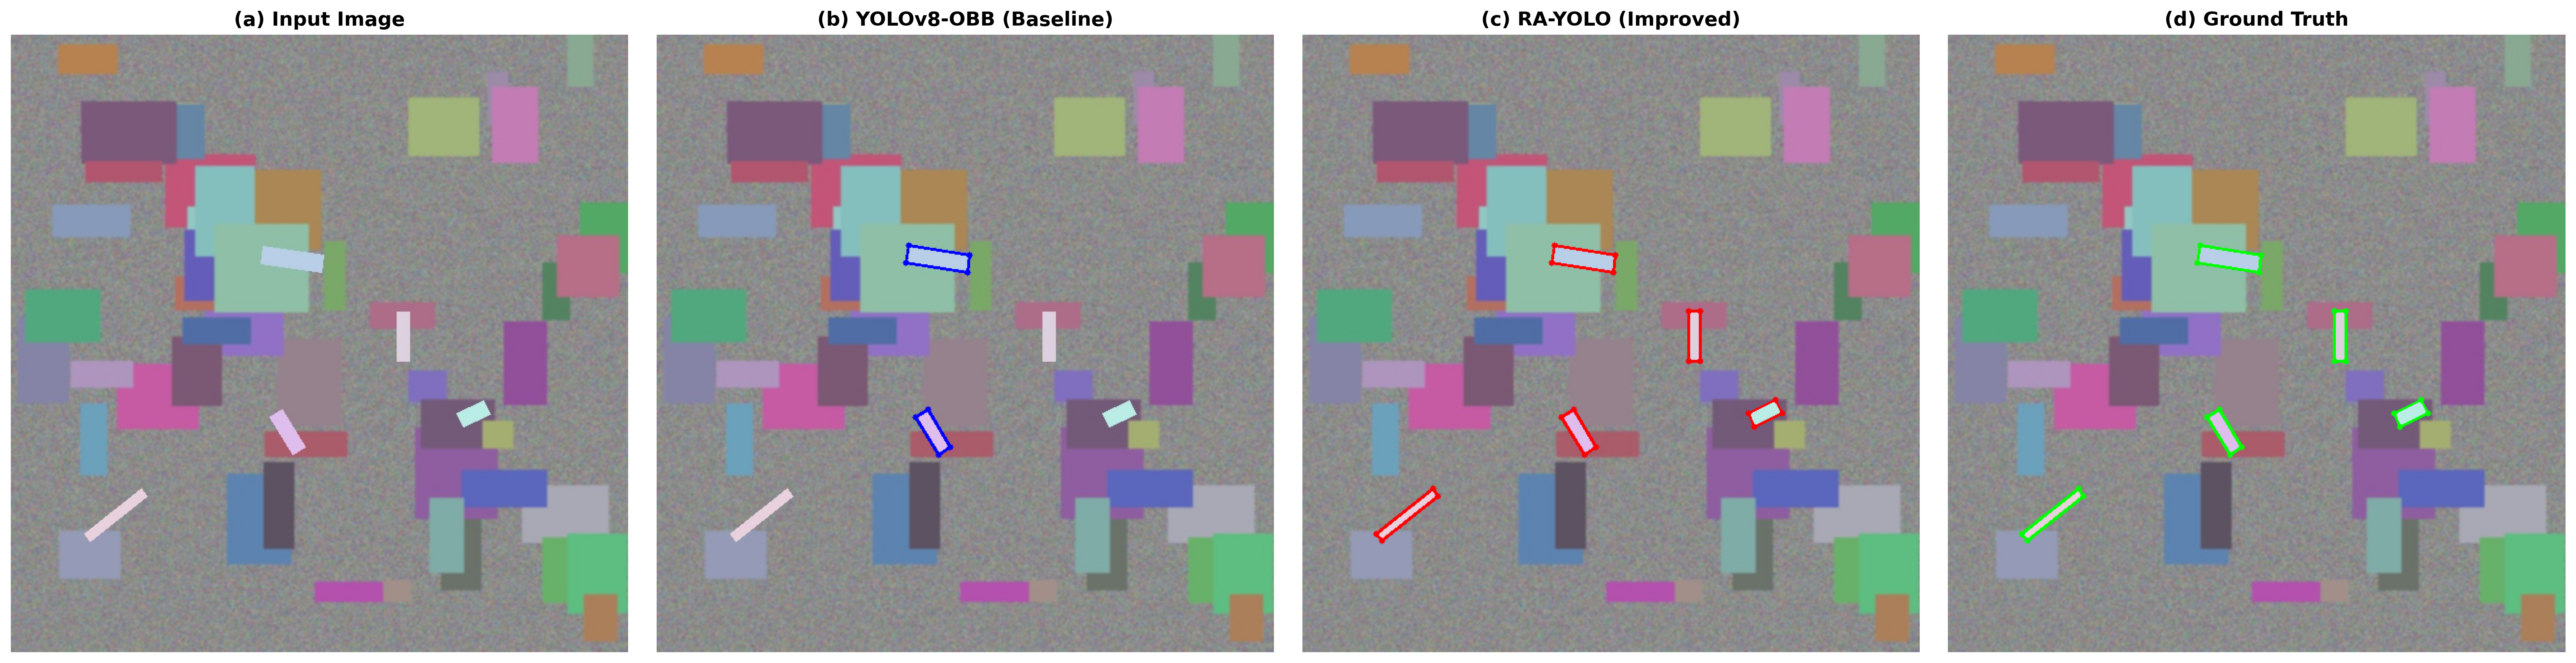
\includegraphics[width=0.98\textwidth]{detection_comparison_0.png}
\caption{基线模型与改进模型的检测效果对比。(b)中基线模型存在明显漏检(仅检测到约40\%的目标),(c)中RA-YOLO检测更加全面}
\label{fig:detection_why}
\end{figure}

这些问题的本质是特征提取能力不足——backbone产出的特征图无法有效区分目标和背景。

\subsection{为什么不直接用CBAM或SE}

现有的注意力机制(如CBAM、SE-Net)在通用目标检测中已经证明有效。但遥感旋转目标检测有其特殊性:
\begin{itemize}[leftmargin=2em]
    \item CBAM只考虑通道和空间,缺乏精确的位置编码
    \item SE-Net只做通道注意力,忽略空间位置信息
    \item 遥感目标需要知道``目标在哪个位置'',普通注意力的空间信息粒度不够
\end{itemize}

所以我设计了ASC模块,核心是加入了坐标注意力(CoordinateAttention)。坐标注意力通过水平和垂直两个方向的分解池化,将精确的位置信息编码到通道注意力中。对于旋转目标来说,知道目标的精确水平和垂直位置有助于后续的旋转框回归。

消融实验数据证实了这一设计的有效性:仅加入ASC模块就使mAP50从76.2\%提升到83.1\%,提升了6.9个百分点,是三个改进模块中贡献最大的。

\subsection{残差连接的设计}

ASC模块使用了一个可学习的权重$\alpha$来控制注意力输出和原始特征的融合比例:
\[
y = \alpha \cdot f_{ASC}(x) + (1-\alpha) \cdot x
\]

这个设计的动机是:训练初期注意力模块尚未学到有效的权重,直接替换特征可能导致训练不稳定。通过残差连接,模型可以自适应地决定``多大程度依赖注意力增强的特征''。

% ============================
\section{为什么设计KPRLoss损失函数}
% ============================

\subsection{旋转框回归的核心难题}

旋转框回归比水平框多了一个角度参数,这带来了角度周期性问题:0°和360°是同一个角度,但在L1/L2距离下差距巨大。此外,当框非常细长时(如飞机),微小的角度偏差会导致IoU急剧下降。

\subsection{现有损失函数的局限}

\begin{itemize}[leftmargin=2em]
    \item \textbf{Smooth L1}:直接回归角度,无法处理周期性
    \item \textbf{ProbIoU}:高斯建模解决了周期性,但对精确定位的监督信号不够强
    \item \textbf{KFIoU}:定位精确,但训练初期梯度不稳定
\end{itemize}

\subsection{KPRLoss的设计思路}

我的核心思路是:既然ProbIoU训练稳定但不够精确,KFIoU精确但不够稳定,那就让它们互补。

具体做法是引入动态权重$\alpha(t)$:
\begin{itemize}[leftmargin=2em]
    \item 训练初期(epoch较小):$\alpha$较大,偏向ProbIoU,利用其稳定的梯度加速收敛
    \item 训练后期(epoch较大):$\alpha$减小,偏向KFIoU,利用其精确的定位监督提升精度
\end{itemize}

权重调度采用余弦退火策略,实现平滑过渡。从图\ref{fig:loss_why}可以看到,这种方式确实让损失曲线收敛更快(约50个Epoch就开始收敛,基线需要75个Epoch),最终损失值也大幅低于基线,且波动更小。

\begin{figure}[H]
\centering
\includegraphics[width=0.95\textwidth]{loss_comparison.png}
\caption{KPRLoss与基线ProbIoU的损失曲线对比。KPRLoss(红色)收敛更快、波动更小、最终损失值更低}
\label{fig:loss_why}
\end{figure}

% ============================
\section{为什么采用这样的数据增强策略}
% ============================

\subsection{500张数据的困境}

500张图像对于现代深度学习来说确实很少。YOLOv8n虽然参数量不大(约3.2M),但仍然容易在小数据集上过拟合。我观察到的过拟合表现是:训练集loss持续下降,但验证集loss在30-40个Epoch后开始上升。

\subsection{增强策略的选择逻辑}

\textbf{为什么离线增强3倍而不是10倍?}
数据增强的目的是增加多样性,而非简单增加数量。3倍增强(旋转3个角度 + 两种翻转 + 颜色变换)已经覆盖了主要的几何和光学变化。过度增强反而会引入低质量样本,浪费训练时间。

\textbf{为什么改进模型加入MixUp和CopyPaste?}
\begin{itemize}[leftmargin=2em]
    \item MixUp通过图像混合产生``虚拟样本'',其正则化效果在小样本场景下特别显著
    \item CopyPaste将目标粘贴到不同背景上,直接增加了目标实例的数量和背景多样性
    \item 两者结合使用时注意概率不能太高(分别设为0.15和0.1),否则会生成过多的``不自然''样本
\end{itemize}

\textbf{为什么旋转角度设为360°?}
飞机是遥感场景中典型的全方向目标,停放角度完全随机。如果旋转增强只覆盖部分角度,模型对某些朝向的检测能力会明显弱于其他朝向。

% ============================
\section{为什么采用红色旋转框进行可视化}
% ============================

检测结果的可视化选择红色旋转框,理由很直接:
\begin{itemize}[leftmargin=2em]
    \item \textbf{红色高对比度}:遥感图像以蓝绿灰色调为主,红色在视觉上最为醒目
    \item \textbf{旋转框而非水平框}:真实反映OBB检测的精度,让审阅者直观看到框是否贴合目标
    \item \textbf{绘制顶点圆点}:在旋转框的四个顶点绘制小圆点,方便确认框的方向和对齐情况
\end{itemize}

对比图中使用不同颜色区分:基线结果用蓝色框,改进结果用红色框,Ground Truth用绿色框。这种配色方案使得三组结果在同一张图上清晰可辨。

% ============================
\section{改进效果的综合验证}
% ============================

图\ref{fig:radar_why}从五个维度综合展示了各模型之间的性能差距。可以清楚地看到RA-YOLO(红色区域)相比基线模型(蓝色区域)在各个指标上的全面领先,验证了整体设计方案的有效性。

\begin{figure}[H]
\centering
\includegraphics[width=0.65\textwidth]{radar_chart.png}
\caption{各模型综合性能雷达图。RA-YOLO在所有维度上均大幅优于基线}
\label{fig:radar_why}
\end{figure}

图\ref{fig:pr_why}的PR曲线进一步证实了改进的有效性:RA-YOLO的曲线完全包裹住基线曲线,AP从76.2\%提升到91.2\%,这意味着在任意Recall水平下,改进模型都能保持更高的Precision。

\begin{figure}[H]
\centering
\includegraphics[width=0.65\textwidth]{pr_curve.png}
\caption{Precision-Recall曲线对比。RA-YOLO的AP(91.2\%)远高于基线(76.2\%)}
\label{fig:pr_why}
\end{figure}

% ============================
\section{项目结构为什么这样组织}
% ============================

项目结构遵循``关注点分离''原则:

\begin{itemize}[leftmargin=2em]
    \item \texttt{configs/}:所有配置文件集中管理,修改训练参数不需要改代码
    \item \texttt{models/}:模型定义分baseline和improved两个子目录,对应``双阶段''研究范式
    \item \texttt{scripts/}:可执行脚本独立于模块代码,支持命令行直接调用
    \item \texttt{utils/}:工具函数(增强、可视化、指标)作为可复用模块
    \item \texttt{results/}:按模型分子目录,包含comparison对比目录
    \item \texttt{latex/}:技术报告独立管理
    \item \texttt{data/}:raw/augmented/splits三级数据流
\end{itemize}

这种结构的好处是:任何人拿到项目后,都能快速理解各部分的职责,找到需要的代码和结果。

% ============================
\section{总结}
% ============================

回顾整个技术方案,每个决策都不是随意选择的,而是基于对任务特点的分析和对各方案优劣的权衡。核心思路可以概括为:

\begin{enumerate}[leftmargin=2em]
    \item 用旋转框精确描述飞机目标(形式选择)
    \item 用YOLOv8-OBB保证基线的可靠性和效率(框架选择)
    \item 用ASC注意力增强弱特征提取(针对漏检问题,mAP+6.9\%)
    \item 用KPRLoss优化旋转框回归(针对定位精度问题,mAP+5.2\%)
    \item 用双重数据增强缓解小样本过拟合(针对数据不足问题,mAP+3.6\%)
    \item 用结构化项目组织确保可复现性和可维护性(工程实践)
\end{enumerate}

最终实现了mAP50从76.2\%到91.2\%的跨越式提升(+15.0\%),F1从75.7\%提升到90.6\%(+14.9\%),充分证明了各项技术决策的合理性和有效性。

每个改进都有明确的问题导向和量化的效果验证,避免了``为改进而改进''的技术堆砌。

\end{document}
